\subsection{Iteration \#4}
I iteration 4 ønskes det at udvide systemet med anti kollision. Inden tilføjelsen af anti kollision kan dronen udelukkende flyve i områder uden forhindringer. Men med tilføjelsen af anti kollision vil det være muligt at flyve med dronen i normale områder med forskellige forhindringer. Hvordan systemet er tiltænkt at bruges beskrives i user story nedenfor:


\subsubsection*{User story}
Under flyvning kontrolleres det løbende hvorvidt der er et objekt foran dronen. Hvis der detekteres et objekt foran dronen, skal dronen holde om med at flyve fremad. I stedet skal dronen dreje horisontalt indtil der ikke længere er et objekt foran den. Når der er frit foran dronen fortsættes den afbrudte flyvning. 
Bruger af systemet har ingen direkte kontakt med anti kollisionssystemet. For bruger ses anti kollision blot som en ekstra feature, som gør dronen i stand til at flyve uden at kollidere med objekter foran sig.
 
%kommentar
\begin{figure}[H]
	\centering
	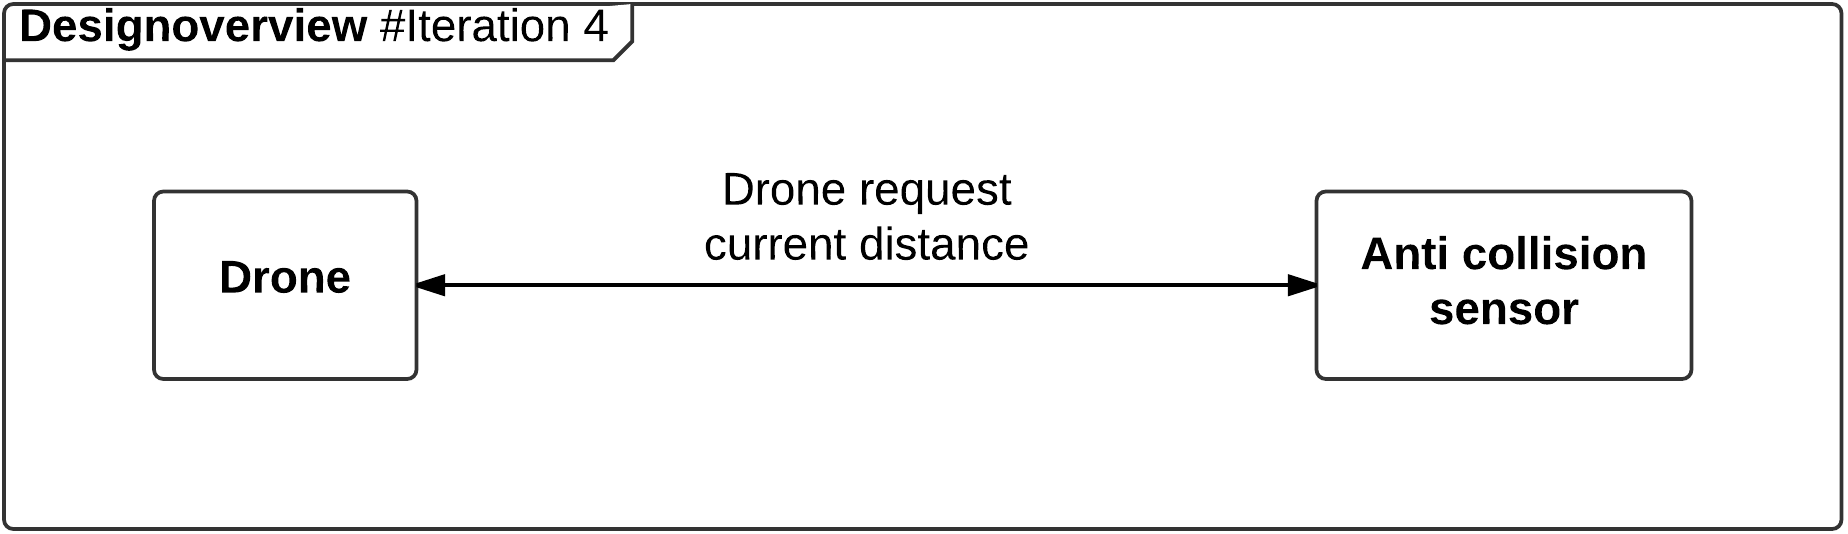
\includegraphics[width=1\textwidth]{Billeder/design_overview/design_overview_iteration4.png}
	\vspace{-.5cm}
	\caption{Designoverview \#iteration 4}
	\label{fig:design_overview_UC4}
\end{figure}


\newpage
\subsubsection*{Sekvens diagram}
\vspace{-0.2cm}
På sekvensdiagrammet vises de klasser der indgår og bruges i fjerde iteration. 
På diagrammet vises det hvordan afstanden til eventuelle objekter foran dronen kontrolleres. Hvis afstanden til et objekt er under den definerede kollisionsgrænse stoppes dronens fremdrift og der skiftes orientering. 


%kommentar
\begin{figure}[H]
	\centering
	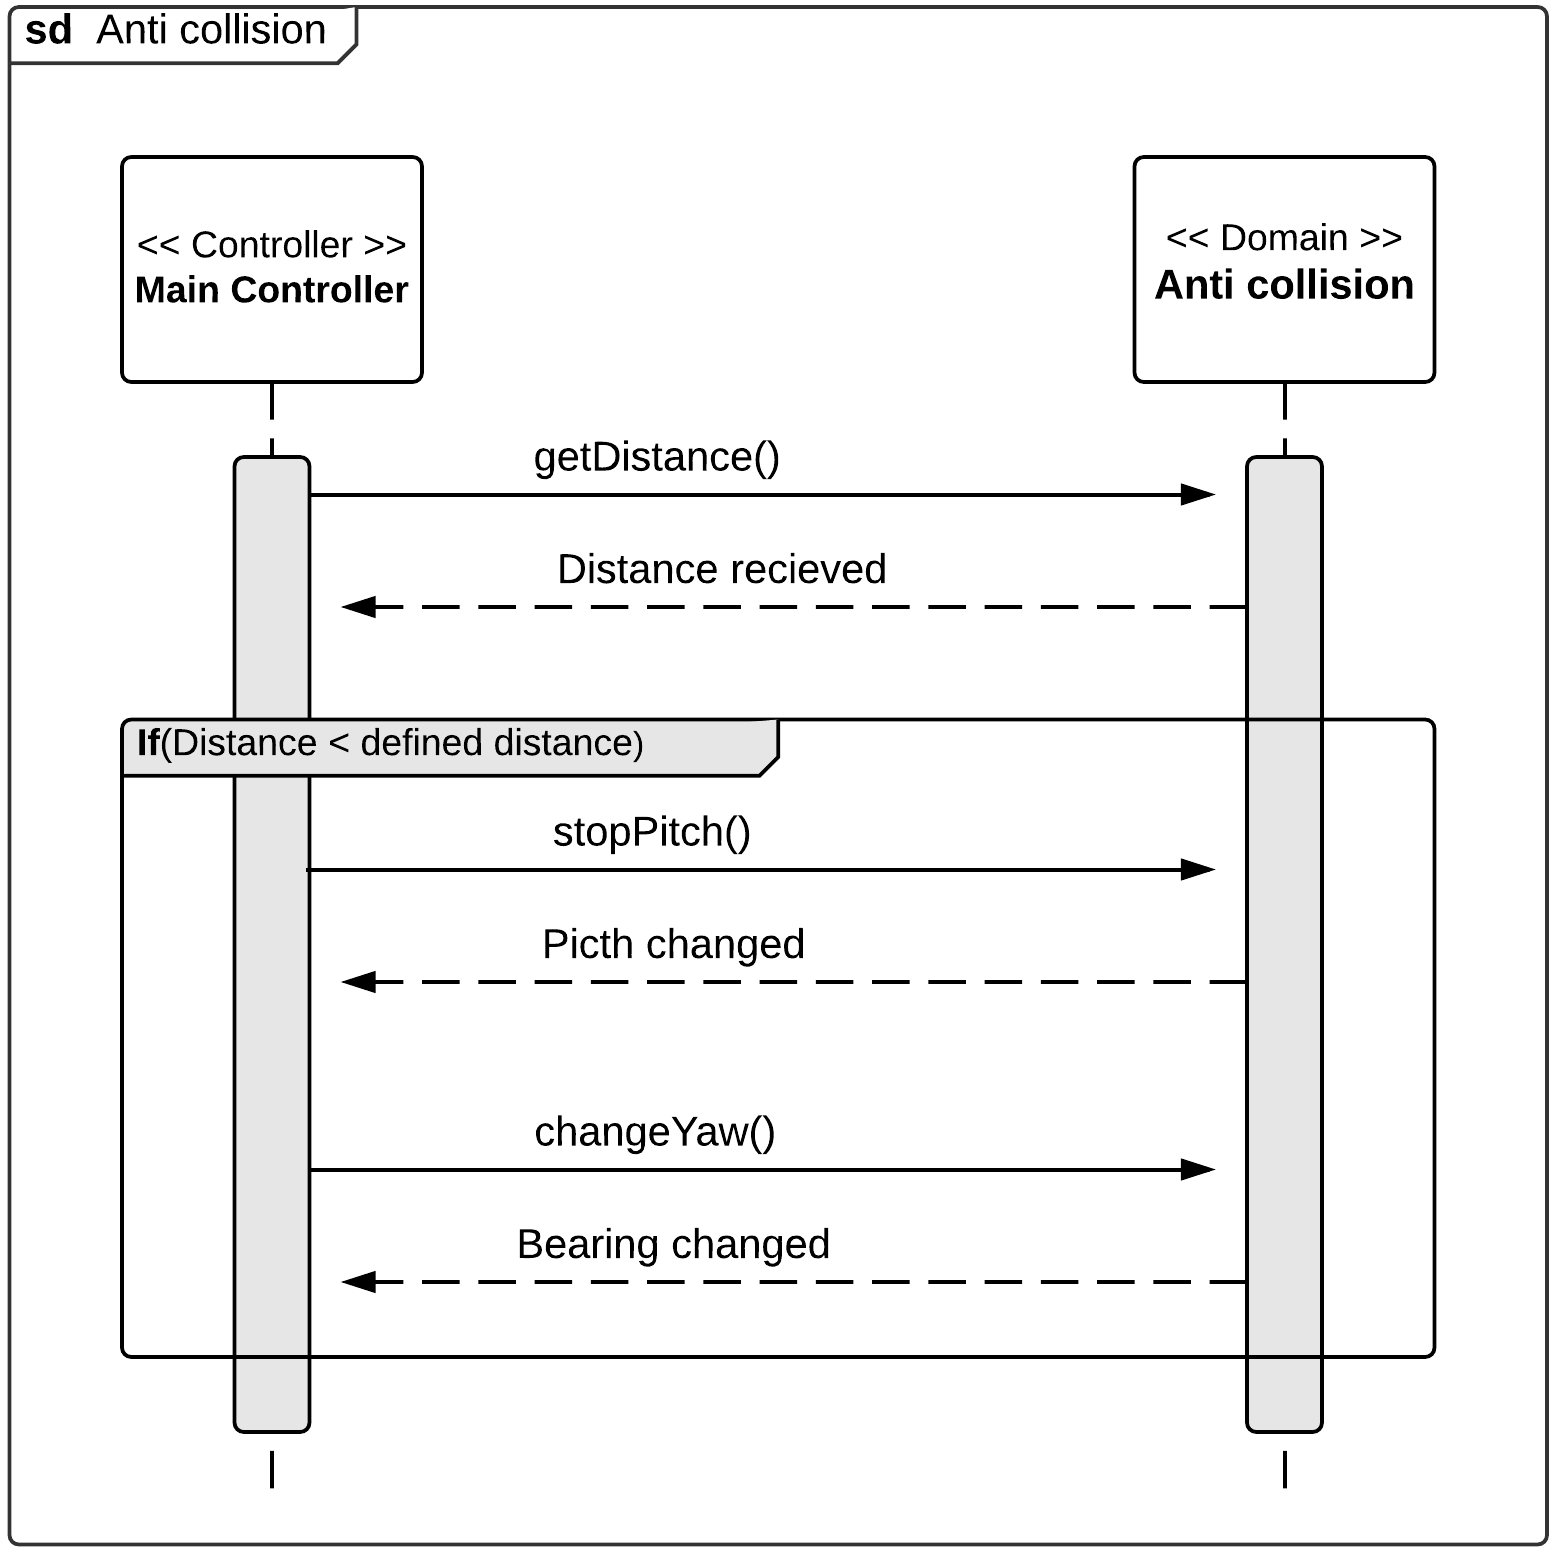
\includegraphics[width=0.8\textwidth]{Billeder/sekvens/sekvens_iteration4}
	\caption{Sekvens diagram \#iteration 4}
	\label{fig:Sekvens_diagram_iteration4}
\end{figure}



\subsubsection*{State machine diagram}
\vspace{-0.2cm}

I state machine diagrammet på figur \ref{fig:Statemachine_iteration4}, vises de to states der eksisterer i iteration 4. Desuden vises hvordan flowet imellem de to states ser ud.


%kommentar
\begin{figure}[H]
	\centering
	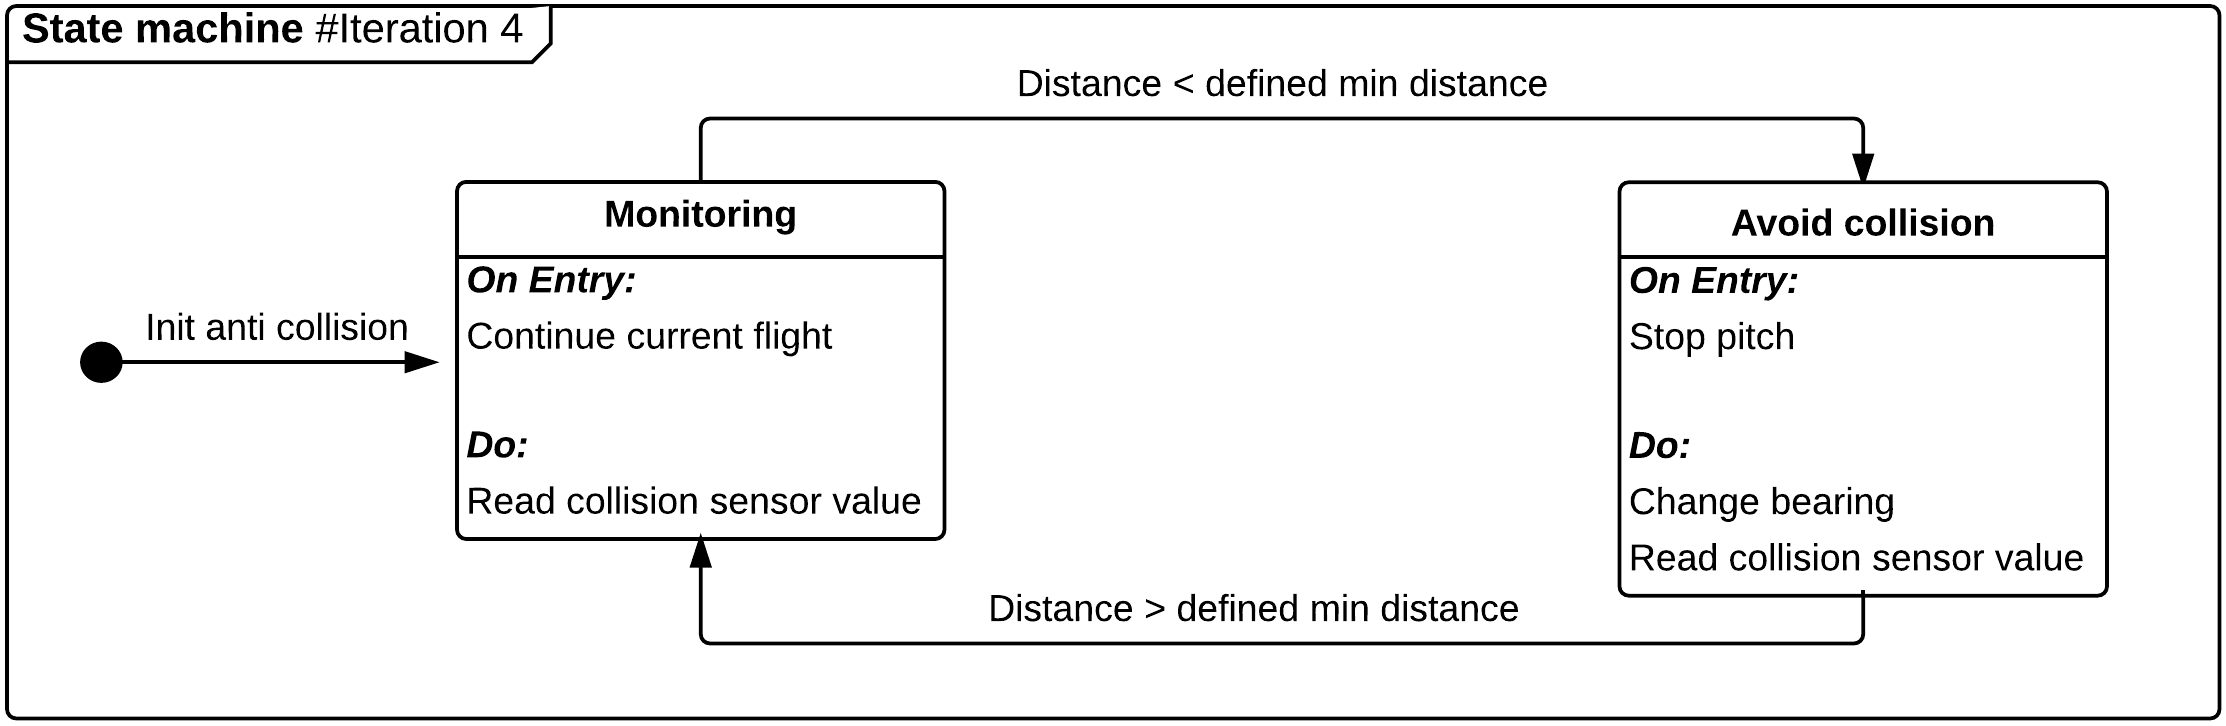
\includegraphics[width=1\textwidth]{Billeder/statemachine/State_iteration4.png}
	\vspace{-0.5cm}
	\caption{Statemachine \#iteration 4}
	\label{fig:Statemachine_iteration4}
\end{figure}



\subsubsection*{Klasse diagram}
\vspace{-0.1cm}

%kommentar
\begin{figure}[H]
	\centering
	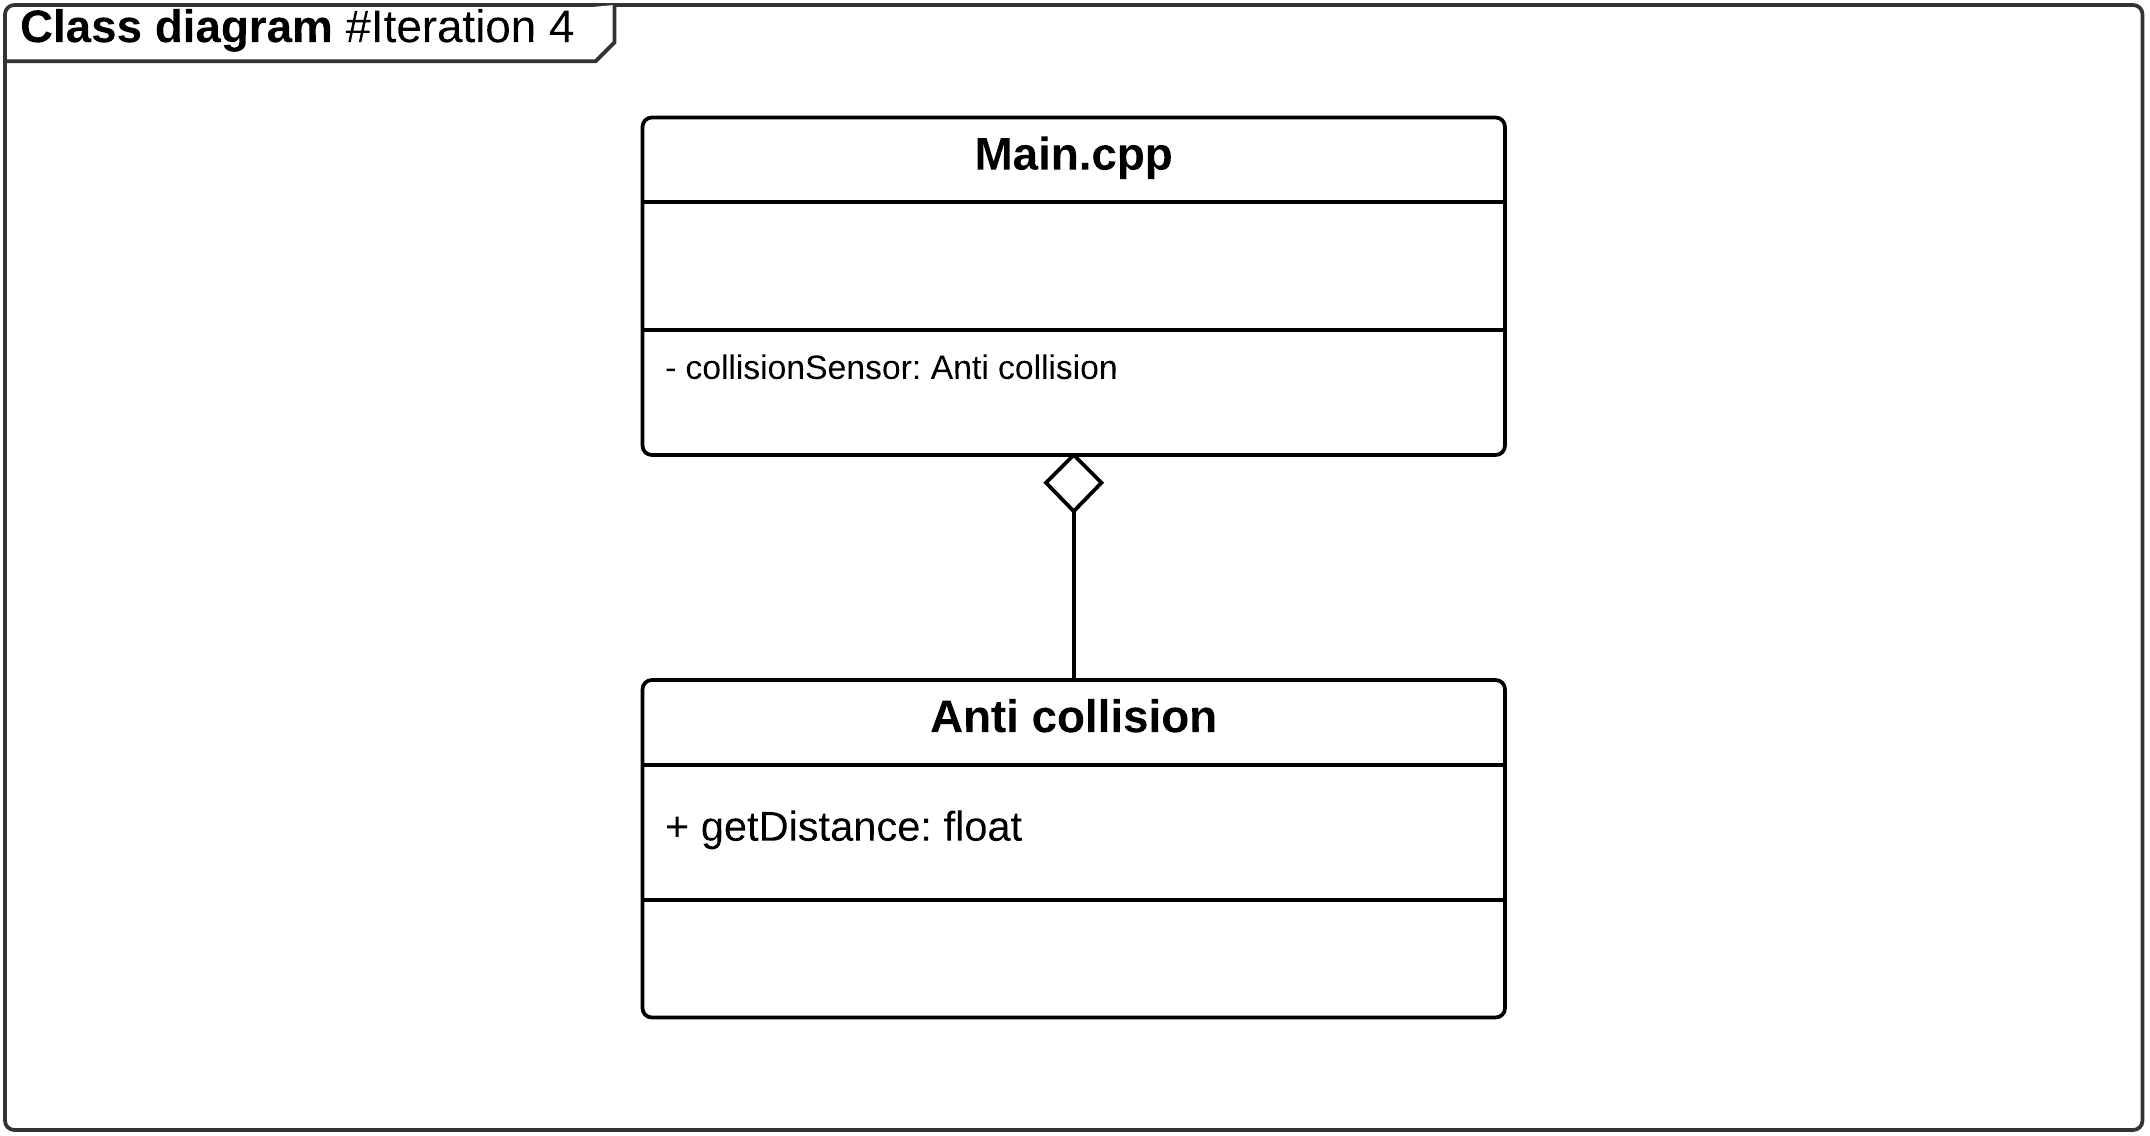
\includegraphics[width=1\textwidth]{Billeder/klasse_diagrammer/classdiagram_iteration4.png}
	\vspace{-0.5cm}
	\caption{Klasse diagram \#iteration 4}
	\label{fig:classDiagram_iteration4}
\end{figure}


\textbf{Main.cpp} \\
Main.cpp filen bruges til at sætte arduino board korrekt op, bla. sættes baudrate på de forskellige serielle forbindelser. Desuden bruges Main.cpp til at kalde og eksekverer forskellige klasse, objekter og funktioner.


\textbf{Anti collision} \\
Module\_3G er ansvarlig for alt kommunikation mellem drone og server. I klassen bruges to forskellige slags http request. Når der ønskes at trække information fra sever til drone gøres der brug af GET request mens der gøres brug af PUT request når dronen ønsker at informere server om ny lokation.
